\section{Movement}

\begin{multicols}{2}


\section*{Human Skeleton}


\subsection{Paper Skeleton} % VSO 44

\begin{center}
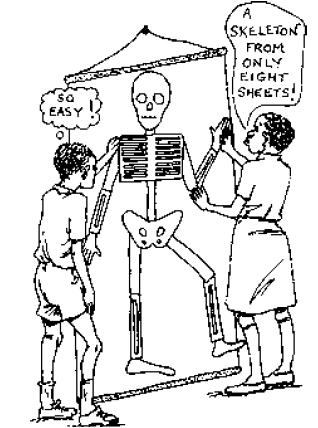
\includegraphics[width=0.4\textwidth]{./img/source/skeleton-full.png}
\end{center}
Construct a paper skeleton as shown using 8 sheets of A4 paper. Pin or staple the skeleton together or mount it on a hanging mat.
%\begin{description*}
%%\item[Subtopic:]{}
%\item[Materials:]{8 sheets of paper}
%%\item[Setup:]{}
%\item[Procedure:]{To make the paper skeleton
%shown here you will need 8 pages
%of A4 paper or pages from a large
%writing book used by students.
%Fold and cut out the shapes as
%illustrated for each part of the
%body. The final result should look
%like the one shown.}
%%\item[Hazards:]{}
%%\item[Questions:]{}
%%\item[Observations:]{}
%%\item[Theory:]{}
%%\item[Applications:]{}
%\item[Notes:]{Pin or staple the skeleton together or mount it on a hanging mat.}
%\end{description*}

\subsubsection{Skull and Pelvis}

\begin{center}
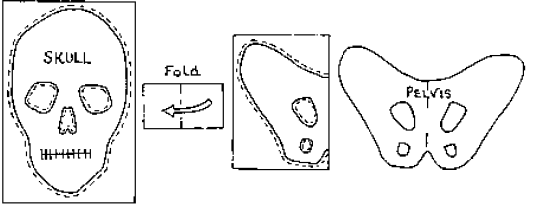
\includegraphics[width=0.49\textwidth]{./img/source/skeleton-skull-pelvis.png}
\end{center}

\begin{description*}
%\item[Subtopic:]{}
%\item[Materials:]{}
%\item[Setup:]{}
\item[Skull:]{Cut around the dotted line after
drawing. The teeth and mouth
can be cut without removing any
paper.}
\item[Pelvis:]{Draw half of the pelvis and cut out the basic shape when the paper is
folded}
%\item[Questions:]{}
%\item[Observations:]{}
%\item[Theory:]{}
%\item[Applications:]{}
%\item[Notes:]{}
\end{description*}

\columnbreak

\subsubsection{Limbs}

\begin{center}
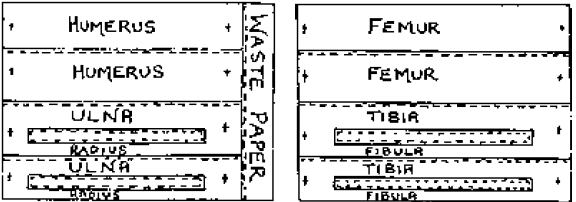
\includegraphics[width=0.49\textwidth]{./img/source/skeleton-limbs.png}
\end{center}
The lower limbs are cut out from one piece of paper. The upper limbs
all fit onto another piece.
%\begin{description*}
%%\item[Subtopic:]{}
%%\item[Materials:]{}
%%\item[Setup:]{}
%%\item[Procedure:]{}
%%\item[Hazards:]{}
%%\item[Questions:]{}
%%\item[Observations:]{}
%%\item[Theory:]{}
%%\item[Applications:]{}
%%\item[Notes:]{}
%\end{description*}

\subsubsection{Rib Cage}

\begin{center}
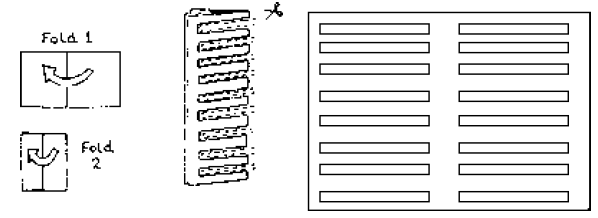
\includegraphics[width=0.49\textwidth]{./img/source/skeleton-ribs.png}
\end{center}
Fold the paper twice and then cut along alternate lines. Use a ruler to
measure accurately if you want to have the exact number of ribs. You
can cut the ribs out of the paper lengthwise instead.
%\begin{description*}
%%\item[Subtopic:]{}
%%\item[Materials:]{}
%%\item[Setup:]{}
%%\item[Procedure:]{}
%%\item[Hazards:]{}
%%\item[Questions:]{}
%%\item[Observations:]{}
%%\item[Theory:]{}
%%\item[Applications:]{}
%%\item[Notes:]{}
%\end{description*}

\subsubsection{Backbone}

\begin{center}
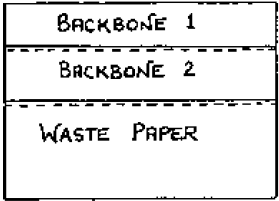
\includegraphics[width=0.2\textwidth]{./img/source/skeleton-backbone.png}
\end{center}
Cut out 2 strips for the backbone
to give extra strength. 
%Stick one
piece to each side of the skeleton.
%\begin{description*}
%%\item[Subtopic:]{}
%%\item[Materials:]{}
%%\item[Setup:]{}
%%\item[Procedure:]{}
%%\item[Hazards:]{}
%%\item[Questions:]{}
%%\item[Observations:]{}
%%\item[Theory:]{}
%%\item[Applications:]{}
%%\item[Notes:]{}
%\end{description*}

\subsubsection{Hands and Feet}

\begin{center}
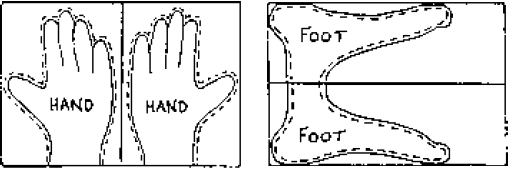
\includegraphics[width=0.49\textwidth]{./img/source/skeleton-hands-feet.png}
\end{center}
Fold the paper in half and draw around a hand. Use
another piece of paper for the feet.
%\begin{description*}
%%\item[Subtopic:]{}
%%\item[Materials:]{}
%%\item[Setup:]{}
%%\item[Procedure:]{}
%%\item[Hazards:]{}
%%\item[Questions:]{}
%%\item[Observations:]{}
%%\item[Theory:]{}
%%\item[Applications:]{}
%%\item[Notes:]{}
%\end{description*}

\subsection{Robotic Hand}

\begin{center}
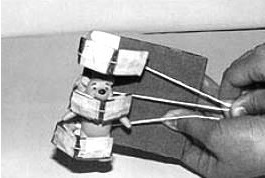
\includegraphics[width=0.49\textwidth]{./img/robotic-hand-use.jpg}
\end{center}

\begin{description*}
%\item[Subtopic:]{}
\item[Materials:]{Rubber bands, straws, cardboard, string, masking tape, scissors}
%\item[Setup:]{}
%\item[Procedure:]{}
%\item[Hazards:]{}
%\item[Questions:]{}
%\item[Observations:]{}
%\item[Theory:]{}
%\item[Applications:]{}
%\item[Notes:]{}
\end{description*}

\subsubsection{Hand Structure}

\begin{center}
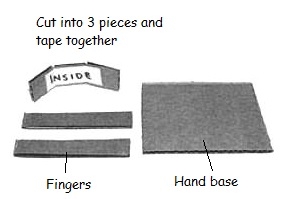
\includegraphics[width=0.49\textwidth]{./img/robotic-hand-1.jpg}
\end{center}

\begin{description*}
%\item[Subtopic:]{}
%\item[Materials:]{}
%\item[Setup:]{}
\item[Procedure:]{Cut a piece of cardboard about 10~cm $\times$ 10~cm. This is the ``palm'' of the hand. Cut three pieces of cardboard about 2 cm $\times$ 9 cm. These are the ``fingers''. Cut one finger into three equal pieces. Place the three finger pieces back together and put a piece of tape over the two
finger joints. Label the tape ``inside''.}
%\item[Hazards:]{}
%\item[Questions:]{}
%\item[Observations:]{}
%\item[Theory:]{}
%\item[Applications:]{}
%\item[Notes:]{}
\end{description*}

\columnbreak

\subsubsection{Fingers}

\begin{center}
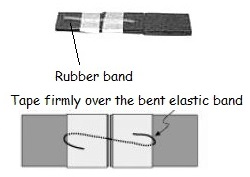
\includegraphics[width=0.45\textwidth]{./img/robotic-hand-finger.jpg}
\end{center}

\begin{description*}
%\item[Subtopic:]{}
%\item[Materials:]{}
%\item[Setup:]{}
\item[Procedure:]{Cut a piece of elastic about 5 cm long. Turn the finger over (inside facing down) and place the elastic across the middle of the first joint. Tape the elastic on either side of the joint, leaving the ends of the elastic untaped (rip tape to make it thin). Bend the ends of the elastic as shown and tape firmly. This will help prevent the elastic from slipping. Repeat for the second joint.}
%\item[Hazards:]{}
%\item[Questions:]{}
%\item[Observations:]{}
%\item[Theory:]{}
%\item[Applications:]{}
%\item[Notes:]{}
\end{description*}

\subsubsection{Attach Fingers}

\begin{center}
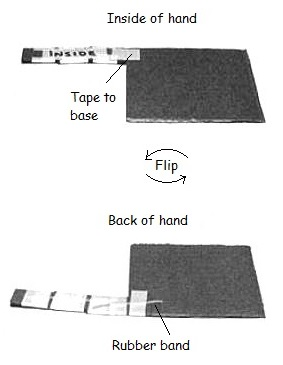
\includegraphics[width=0.45\textwidth]{./img/robotic-hand-3.jpg}
\end{center}

\begin{description*}
%\item[Subtopic:]{}
%\item[Materials:]{}
%\item[Setup:]{}
\item[Procedure:]{Tape the finger (inside up) onto the palm. Turn the hand over and fasten the last finger joint to the palm using the same method as above.}
%\item[Hazards:]{}
%\item[Questions:]{}
%\item[Observations:]{}
%\item[Theory:]{}
%\item[Applications:]{}
%\item[Notes:]{}
\end{description*}

\columnbreak

\subsubsection{Moving Joints}

\begin{center}
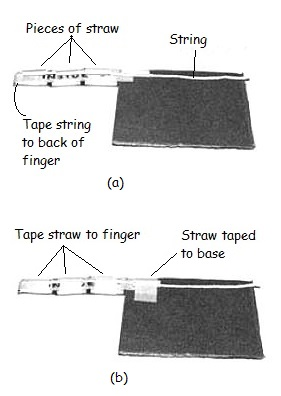
\includegraphics[width=0.49\textwidth]{./img/robotic-hand-4.jpg}
\end{center}

\begin{description*}
%\item[Subtopic:]{}
%\item[Materials:]{}
%\item[Setup:]{}
\item[Procedure:]{Cut a piece of string about 35 cm long and tape one end firmly over the end of
the finger. Cut four pieces of straw each about 2 cm long and thread them onto the string. Tape three of the straws in the middle of each of the finger sections. Tape the last straw to the palm as shown. }
%\item[Hazards:]{}
%\item[Questions:]{}
%\item[Observations:]{}
%\item[Theory:]{}
%\item[Applications:]{}
%\item[Notes:]{}
\end{description*}

\subsubsection{Completing the Hand}

\begin{center}
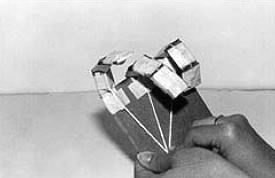
\includegraphics[width=0.45\textwidth]{./img/robotic-hand-final.jpg}
\end{center}

\begin{description*}
%\item[Subtopic:]{}
%\item[Materials:]{}
%\item[Setup:]{}
\item[Procedure:]{Repeat the steps above for the last two fingers. When finished, operate the hand by pulling the strings. You should be able to pick up empty soda cans and other light objects with your hand.}
%\item[Hazards:]{}
%\item[Questions:]{}
%\item[Observations:]{}
%\item[Theory:]{}
%\item[Applications:]{}
%\item[Notes:]{}
\end{description*}

%==================================================================================================%

\section*{Joints}


\subsection{Ball and Socket}

\begin{center}
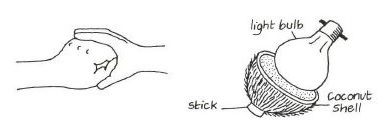
\includegraphics[width=0.45\textwidth]{./img/vso/ball-socket.jpg}
\end{center}

\begin{description*}
%\item[Subtopic:]{}
\item[Materials:]{Light bulb, coconut shell, stick}
%\item[Setup:]{}
\item[Procedure:]{The hip joint, which allows the
thigh to move, is a ball and socket
joint. You can demonstrate such a
joint by cupping your hands or
making one as shown.}
%\item[Hazards:]{}
%\item[Questions:]{}
%\item[Observations:]{}
%\item[Theory:]{}
%\item[Applications:]{}
%\item[Notes:]{}
\end{description*}

\subsection{Hinge Joint}

\begin{center}
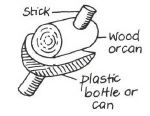
\includegraphics[width=0.3\textwidth]{./img/vso/hinge-joint.jpg}
\end{center}

\begin{description*}
%\item[Subtopic:]{}
\item[Materials:]{Stick, round piece of wood or can, plastic bottle or can}
%\item[Setup:]{}
\item[Procedure:]{The elbow and knee are both
hinge joints and allow movement
in only one direction - like a
hinge. You can make a model of a
hinge joint as shown.}
%\item[Hazards:]{}
%\item[Questions:]{}
%\item[Observations:]{}
%\item[Theory:]{}
%\item[Applications:]{}
%\item[Notes:]{}
\end{description*}

\subsection{Sliding Joint}

\begin{center}
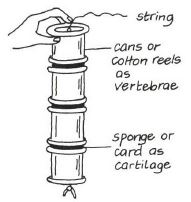
\includegraphics[width=0.35\textwidth]{./img/vso/sliding-joint.jpg}
\end{center}

\begin{description*}
%\item[Subtopic:]{}
\item[Materials:]{String, cans/cotton reels, sponge or card}
%\item[Setup:]{}
\item[Procedure:]{The joints between vertebrae
allow movement of the spine.
Make a model of the spine as
shown.}
%\item[Hazards:]{}
%\item[Questions:]{}
%\item[Observations:]{}
%\item[Theory:]{}
%\item[Applications:]{}
%\item[Notes:]{}
\end{description*}

%==================================================================================================%

\section*{Muscles}


\subsection{Forearm Lever}

\begin{center}
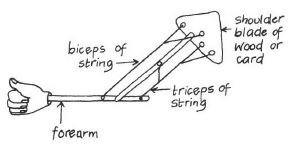
\includegraphics[width=0.49\textwidth]{./img/vso/forearm.jpg}
\end{center}

\begin{description*}
%\item[Subtopic:]{}
\item[Materials:]{Card, string, 2 strong straight sticks}
%\item[Setup:]{}
\item[Procedure:]{Make a model of the forearm as
shown.}
%\item[Hazards:]{}
%\item[Questions:]{}
\item[Observations:]{Notice that the arm
can only be bent by shortening
one `muscle' at a time.}
\item[Theory:]{Muscles can only pull, which in turn causes the motion of complementary muscle groups.}
%\item[Applications:]{}
\item[Notes:]{Try using rubber bands
instead of string.}
\end{description*}

\subsection{Muscles Work in Pairs}

\begin{center}
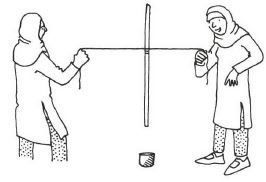
\includegraphics[width=0.45\textwidth]{./img/vso/muscle-pairs.jpg}
\end{center}

\begin{description*}
%\item[Subtopic:]{}
\item[Materials:]{Rod, rope/string, small tin}
%\item[Setup:]{}
\item[Procedure:]{Tie the string to the rod as shown
and ask pairs of students to
manoeuvre the stick into the tin,
or onto a chalk mark on the floor.
}
%\item[Hazards:]{}
%\item[Questions:]{}
%\item[Observations:]{}
\item[Theory:]{The rope can only pull the rod,
not push it. Muscles can only pull
as well.}
%\item[Applications:]{}
%\item[Notes:]{}
\end{description*}

\subsection{Effect of Load on Muscle}

\begin{center}
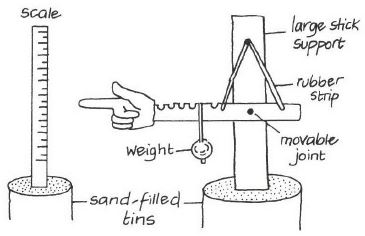
\includegraphics[width=0.49\textwidth]{./img/vso/load-muscle.jpg}
\end{center}

\begin{description*}
%\item[Subtopic:]{}
\item[Materials:]{2 tins filled with sand, ruler, rubber band, 2 strong sticks, weights}
%\item[Setup:]{}
\item[Procedure:]{Make a model arm as shown. Use a light weight to begin with and then
increase the load. Discuss what happens to the
muscle as you increase the load
(weights) on the lever (arm) and
the effect of the position of the
weight on the `arm'.
}
%\item[Hazards:]{}
%\item[Questions:]{}
%\item[Observations:]{}
%\item[Theory:]{}
\item[Applications:]{Students should move their arms
to correspond to the model.
Discuss with them where they
usually carry loads on their arms
and why.}
%\item[Notes:]{}
\end{description*}

\subsection{Support of the Spinal Column}

\begin{center}
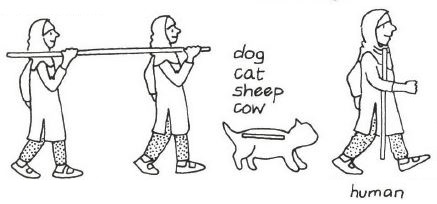
\includegraphics[width=0.45\textwidth]{./img/vso/spine.jpg}
\end{center}

\begin{description*}
%\item[Subtopic:]{}
%\item[Materials:]{}
%\item[Setup:]{}
%\item[Procedure:]{}
%\item[Hazards:]{}
%\item[Questions:]{}
%\item[Observations:]{}
\item[Theory:]{The diagrams show the position of the spinal column in relation
to the legs. Ask students to load the
`backbone' by adding weights
to it and discuss the effect on
the joints.
Discuss the role of muscles in
maintaining the posture of
each animal.}
%\item[Applications:]{}
%\item[Notes:]{}
\end{description*}

%==================================================================================================%


\end{multicols}

\pagebreak